\section{Aktueller Stand}

In diesem Kapitel wird auf den aktuellen Stand der Technik und der Marktintegration von Biogas und Biomethan eingegangen. Zusätzlich wird der rechtliche Rahmen erläutert und Hemmnisse aufgezeigt, die den Prozess hin zu einer Flexibilisierung von Biogasanlagen erschweren.


\subsection{Stand der Technik}\label{chap:stateofart}
Das unverarbeitete Rohbiogas ist ein Gasgemisch. Seine Hauptbestandteile sind Methan mit \SIrange{50}{75}{\percent}, Kohlenstoffdioxid mit \SIrange{20}{50}{\percent} und Wasserdampf mit \SIrange{1}{5}{\percent}. Weitere mögliche Bestandteile sind Schwefelwasserstoff, Ammoniak, Stickstoff und Siloxane. Die genaue Zusammensetzung des Biogas ist in erster Linie abhängig von der zur Produktion verwendeten Biomasse \parencite{Rasi09}. Sie bestimmt damit außerdem welche Gasreingungs- und Aufbereitungsverfahren durchgeführt werden müssen, damit es als Biomethan in das deutsche Erdgasnetz eingespeist werden darf. Dabei ist das Hauptziel den Methananteil, und damit den Heizwert, zu erhöhen und die übrigens Bestandteile soweit wie möglich zu reduzieren. Die wichtigsten Anforderungen, gestellt durch den \glspl{DVGW}, sind in \ref{tab:tab_gasgrid_spec} zusammengefasst. Die geringen Anteile von Siloxanen und Ammoniak im Biogas werden oft durch andere Gasreinigungsverfahren entfernt, sodass eine separate Gasreinigung meist nicht nötig ist. \parencite{FNR14}\parencite{KoBi16}
{
\renewcommand{\arraystretch}{1.1}
\begin{table}[H]
	\begin{center}
		\caption{Anforderungen an Gas aus regenerativen Quellen \parencite{FNR14}\parencite{KoBi16}}
		\begin{tabu} to 0.5\textwidth {| X[0.6] | X | X[1.2] |}
\hline
			Komponente  &	zul. Anteil  & Wirkung					\\		
\hline
			\multirow{2}{*}{\ce{CH4}} &	L-Gasnetze: \SI{\geq 90}{\Molpercent}  &	brennbare Gaskomponente	\\
					 &	H-Gasnetze: \SI{\geq 95}{\Molpercent}	&	{}							\\ 
\hline

			\multirow{2}{*}{\ce{CO2}}  	&	L-Gasnetze: \SI{\leq 10}{\Molpercent}  &	vermindert Brennwert	\\
						&	H-Gasnetze: \SI{\leq 5}{\Molpercent}	 &	{}						\\ 

\hline
			\multirow{2}{*}{\ce{H}}     	&	bis Netzdruck \SI{10}{\bar}: \SI{\leq 200}{\mgcubm}	&	Korrosion; Kondensat beschädigt Instrumente und Aggregate	\\
						&	Netzdruck größer \SI{10}{\bar}: \SI{\leq 50}{\mgcubm}	& {}	\\ 
\hline
			\multirow{1}{*}{\ce{H2S}}  	&	\SI{\leq 5}{\mgcubm}  	&	Korrosion			\\
\hline
			\multirow{1}{*}{\ce{NH3}}  	&	k.A.  	&	verringert Zündverhalten			\\
\hline
			
		\end{tabu}
		\label{tab:tab_gasgrid_spec}
	\end{center}
\end{table}
}

% Anzahl Anlagen in Deutschland und wie sie vorgehen

% Schema zeichnen?

Im Folgenden werden Gasaufbereitungsverfahren vorgestellt, deren primärer Zweck es ist Kohlenstoffdioxid aus dem Biogas zu entfernen und damit seinen Brennwert zu erhöhen.
\smallskip


\subsubsection{Absorptionsverfahren}\label{chap:absorp}

{\textbf Kurzer Einleitungssatz noch -} Bei physikalischer Absorption werden unerwünschte Bestandteile eines Gasstroms in einem Flüssigkeitsstrom gelöst. Der Konzentrationsunterschied des gelösten Gases im Lösungsmittel und der Gasphase ist dabei die treibende Kraft für den Stoffübergang. Wenn die abgeschiedenen Gasbestandteile dabei mit dem Lösungsmittel reagieren, spricht man von chemischer Absorption. \parencite{Rasi09} \newline
Das weltweit verbreitetste Verfahren ist die \gls{DWW} mit einem Anteil von \SI{41}{\percent}. Sie basiert auf der physikalischen Absorption von Gasen Wasser. Das Verfahren nutzt dabei aus, dass die Löslichkeit von Methan bei \SI{25}{\degreeCelsius} \SI{26}{\relax} mal schlechter als von Kohlenstoffdioxid. Das Rohbiogas wird unter hohem Druck von \SIrange{8}{10}{\bar} in die flüssige Phase des Absorbers geleitet, wo \ce{CO2} absorbiert wird. Das Lösungsmittel wird anschließend mit Luft in einen Desorber geleitet, wo sich das \ce{CO2} vom Wasser löst. Das Wasser wird anschließend wieder dem Absorber zugeführt. Das Schwachgas, das kleine Mengen von \ce{CH4} enthält muss nachbehandelt werden bevor es in die Atmosphäre geleitet wird.
Die Löslichkeit von Schwefelwasserstoff \ce{H2S} in Wasser ist sogar noch besser, sodass diese Bestandteile ebenfalls aus dem Biogas entfernt werden können. Da \ce{H2S} allerdings umweltschädlich und deshalb nicht in die Atmosphäre geleitet wird, sollte das Biogas vor der \gls{DWW} entschwefelt werden. Wird das beachtet ist der Prozess einer der einfachsten Wege Biogas umweltfreundlich und kostengünstig aufzuwerten. \parencite{KGKK2019} \parencite{BHPT13} \newline
Neben der \gls{DWW} werden auch ähnliche Waschverfahren mit organischen Lösungsmitteln verwendet. Wie bei der \gls{DWW} gibt es eine Absorptionsstufe bei erhöhtem Druck und eine Regenerationsstufe. Die Polyethylenglykol-Dimethylether Waschmittel, bekannt unter den Handelsnamen Genosorb \textsuperscript{\textregistered} oder Selexol \textsuperscript{\textregistered}, weisen eine deutlich höhere \ce{CO2}-Löslichkeit als Wasser auf. So sind kleinere Waschmittelmengen und Absorberabmessungen möglich. Allerdings ist der Regenerationsaufwand der organischen Mittel höher, da sie neben entspannt auch erhitzt werden müssen. In der Regel genügt die Wärmezufuhr aus der Schwachgasbehandlung, sodass kein zusätzliche Energieaufwand nötig ist. \ce{H2S} Absorption ist auch hier technisch möglich, aber nicht sinnvoll wegen derselben Gründe. \parencite{FNR14} \newline
Die Aminwäsche funktioniert nach dem Prinzip der chemischen Absorption. Saure Gasbestandteile im Biogas, \ce{CO2} und potenziell \ce{H2S}, reagieren im Absorber exotherm reversibel mit einer Lösung aus Wasser und Aminen und werden somit chemisch gebunden. Damit die Reaktion nicht in einen Gleichgewichtszustand gerät, besteht ein deutlicher Überfluss an Aminlösung. Die Absorption findet bei einem Druck von \SIrange{1}{2}{\bar} statt und das meist verwendete Amin ist Methyldiethanolamin (MDEA). Die Regeneration des Lösungsmittels findet in einer Stripkolonne statt. Dazu wird es auf \SIrange{120}{160}{\degreeCelsius} aufgeheizt, um die nötige Reaktionswärme aufzubringen. Das gelöste \ce{CO2} wird in einem Kondensator abgekühlt und in die Atmosphäre geleitet. Wie auch bei den anderen Wäscheverfahren würde die Absorption von \ce{H2S} sich negativ auf die Effizienz des Prozesses und auf die Umwelt auswirken. \parencite{BHPT13} \parencite{KGKK2019}


\subsubsection{Membranverfahren}\label{chap:membrane} 

Biogasaufbereitung mithilfe von Membranverfahren nutzen die unterschiedlichen Permeabilitäten von Gasanteilen mithilfe einer semi-permeabelen Membran. Je nach Molekülgröße können manche Bestandteile auf die andere Seite diffundieren. Für Biogasaufbereitung werden Membranen verwendet, die \ce{CO2}, \ce{H2O}, \ce{O2} und \ce{H2S} durchdringen lassen, während \ce{CH4} und \ce{N2} übrig bleiben. Üblich sind drei verschiedene Arten von Membranen, polymerische, anorganische und Mixed-Matrix-Membranen (MMM), die jeweils ihre Vor- und Nachteile besitzen. Die Gas/Gas-Diffusion findet unter hohen Drücken von meist \SIrange{20}{40}{\bar} statt, sodass neben den gewünschten Gasen auch Spuren von \ce{CH4} in das Permeat gelangen. Um dem entgegen zu wirken, werden mehrstufige Prozesse genutzt, um den \ce{CH4}-Anteil zu erhöhen und die Verluste zu verringern. Außerdem werden nun auch Verfahren entwickelt, die das Membranverfahren mit einer Absorption verbinden. Auf einer Seite der Membran befindet sich ein Lösungsmittel, das gasförmiges \ce{CO2} und \ce{H2S}, das von der anderen Seite diffundiert, absorbiert. Das Biogas hat dabei einen leicht erhöhten Druck, damit die Flüssigkeit nicht in die Gasphase gerät. Membranverfahren bieten die Möglichkeit preiswert hohe \ce{CH4}-Konzentrationen zu erreichen. Hier ist allerdings auch dringend zu raten das Biogas vorher zu reinigen, damit die Membran nicht verstopft oder beschädigt wird     \parencite{KGKK2019}


\subsubsection{Druckwechseladsorption}\label{chap:PSA}


\subsubsection{Kryogene Verfahren}\label{chap:kryo}



\subsubsection{Hybridverfahren}\label{chap:hybrid} 


\subsubsection{Bioelektrochemische Methanisierung}\label{chap:bioelectr}


\subsubsection{Biochemische Methanisierung}\label{chap:biochem} 




% ToDo: Je nach eingesetzten Material produzieren die Bakterien Biogas mit einem Methangehalt von 50 bis 75 % https://www.umweltbundesamt.de/themen/wirtschaft-konsum/industriebranchen/biogasanlagen#einfuhrung

\subsection{Stand der Forschung und Entwicklung}


\subsection{Rechtliche Rahmenbedingungen für die Flexibilisierung von Bestandsanlagen}\label{chap:law_theo}

Grundlage für die Förderung von Biogas- und Biomethananlagen bildet das \gls{EEG}. Das \gls{EEG} wurde erstmals im Jahr 2000 in Kraft gesetzt und enthielt bis einschließlich zur Fassung des \gls{EEG} \SI{2012}{\relax} hohe Fördersätze für die Erzeugung von Strom aus Biogas. Dies führte zu einem starken Anstieg der installierten Leistung an Biogasanlagen innerhalb dieser Zeitspanne (s. Abb. \ref{fig:ee-cap_biogas}). Seither gibt es nur noch einen im Vergleich geringeren Zubau an Biogasanlagen. \parencite{DanielGromke2019}\smallskip

Mit dem \gls{EEG} \SI{2014}{\relax} kam es zu einer Einführung neuer Rahmenbedingungen für den Einsatz von Biogas- und Methan. So wurde die Höchstbemessungsleistung (s. Kap. \ref{chap:law_Bem}), die verpflichtende Direktvermarktung (s. Kap. \ref{chap:law_DV}) und die Flexibilitätsprämie für Bestandsanlagen (s. Kap. \ref{chap:law_FP}) implementiert, was zu einem abbremsen des Biogas und -methan Ausbaus führte. Bei der Biogasaufbereitung zu Biomethan kommt erschwerend hinzu, dass die Auszahlung vermiedener Netzentgelte (s. Kap. \ref{chap:law_vN}) im Jahr \SI{2010}{\relax} auf \SI{10}{\Jahre} begrenzt wurde. \parencite{BDEW2019a}


\subsubsection{Höchstbemessungsleistung}\label{chap:law_Bem}

Mit dem \gls{EEG} \SI{2014}{\relax} wurde die Höchstbemessungsleistung eingeführt, wodurch sich die Gegebenheiten auch für Bestandsanlagen verschlechterten. Nach \S 101 Abs. 1 ist die \glqq Höchstbemessungsleistung [...] die höchste Bemessungsleistung der Anlage in einem Kalenderjahr seit dem Zeitpunkt ihrer Inbetriebnahme und vor dem \DTMdate{2014-01-01}.\grqq{} Wobei nach \S 5 Nr. 4 die Bemessungsleistung diejenige Leistung ist, die eine Anlage innerhalb eines Jahres im Durchschnitt erbringt. \parencite{BJV2014a} Die Höchstbemessungsleistung legt fest, bis zu welcher Einspeisung eine Anlage ihre Vergütung nach dem \gls{EEG} erhält. Liegt die Einspeisung einer Anlage über der Höchstbemessungsleistung, so erhält der Betreiber für jede darüber hinausgehende erzeugte \si{\kwh} nur den jeweiligen Monatsmarktwert (Definition nach \S 5 Nr. 25). \parencite{Loibl2014}\smallskip

Die Einführung der Höchstbemessungsleistung hat somit massiven Einfluss auf die Erweiterungsmöglichkeiten von Bestandsanlagen, da es sich wirtschaftlich nicht lohnt, die jährliche Stromerzeugung der Anlage zu erhöhen. Hierdurch wird erzielt, dass sich Erweiterungen auf die Flexibilisierung der Anlage konzentrieren. \parencite{DanielGromke2019}


\subsubsection{Direktvermarktung}\label{chap:law_DV}

Bereits mit dem \gls{EEG} \SI{2012}{\relax} wurde eine verpflichtende Direktvermarktung für Biogas- und Biomethananlagen, die nach dem \DTMdate{2014-01-01} in Betrieb genommen wurden und eine Leistung von mehr als \SI{750}{\kw} aufweisen, eingeführt. Mit dem \gls{EEG} \SI{2014}{\relax} wurde diese auf alle Neuanlagen ab dem \DTMdate{2016-01-01} mit einer Leistung von \SI{100}{\kw} ausgeweitet.\smallskip

Für kleine Anlagen und Bestandsanlagen ist eine Direktvermarktung freiwillig. Allerdings kann die Flexibilitätsprämie (s. Kap. \ref{chap:law_FP}) nur in Anspruch genommen werden, wenn der Strom direktvermarktet wird. Zusätzlichen Anreiz bietet das Marktprämienmodell, da es durch die Managementprämie für regelbare Anlagen zu einer Erhöhung der Einspeiseerlöse um \SI{0.2}{\ctkwh} kommt.\smallskip

Bei diesem Modell setzt sich die Gesamtvergütung, als anzulegender Wert bezeichnet, aus dem technologiespezifischen Monatsmarktwert und der Marktprämie zusammen. Der anzulegende Wert ist dabei fixiert und entspricht der anlagenspezifischen \gls{EEG} Vergütung plus der Managementprämie. Da der Monatsmarktwert schwankt, wird die Marktprämie monatsscharf angepasst, um den anzulegenden Wert konstant zu halten. \parencite{NKGH-DV}


\subsubsection{Flexibilitätsprämie für Bestandsanlagen}\label{chap:law_FP}

Das Ziel der Flexibilitätsprämie ist es, den Anteil an regelbarer Erzeugungsleistung zu erhöhen und stellt den größten Anreiz für Anlagenbetreiber von Bestandsanlagen dar, zusätzliche flexible Anlagenleistung zu installieren. Dabei kann die Flexibilitätsprämie nur für Anlagen in Anspruch genommen werden, die vor dem \DTMdate{2014-08-01} in Betrieb genommen wurden.\smallskip

Nach \S 50b \gls{EEG} können \glqq Betreiber von Anlagen [...] von dem Netzbetreiber eine Prämie für die Bereitstellung zusätzlich installierter Leistung für eine bedarfsorientierte Stromerzeugung (Flexibilitätsprämie) verlangen.\grqq{} Dabei beläuft sich die Flexibilitätsprämie auf \SI{130}{\sieuro} je \si{\kw} zusätzlicher flexibler Anlagenleistung pro Jahr für eine gesamte Förderdauer von \SI{10}{\Jahren}. Voraussetzung hierfür ist die seit dem \gls{EEG} \SI{2014}{\relax} verpflichtende Direktvermarktung des erzeugten Stromes. Zusätzlich muss \glqq{}die Bemessungsleistung der Anlage [...] mindestens das \SI{0.2}{\relax}-fache der installierten Leistung der Anlage\grqq{} betragen (s. Anlage 3 Nummer \rom{1} \gls{EEG} \SI{2017}{\relax}). \parencite{BJV2014} \parencite{DanielGromke2019}\smallskip

Die individuelle Flexibilitätsprämie einer Anlage berechnet sich nach Anlage 3 Nummer \rom{2} \gls{EEG} \SI{2017}{\relax} wie folgt:

\begin{equation}
\begin{split}
	FP & = P_{\text{Zusatz}} \cdot \SI{130}{\Eurkw} \\
	& = \left(P_{\text{Inst}} - f_{\text{Kor}} \cdot P_{\text{Bem}}\right) \cdot \SI{130}{\Eurkw}
\end{split}
\end{equation}

Wobei:

\begin{conditions}
	FP					&		Flexibilitätsprämie						\\
	P_{\text{Zusatz}}	&		Zusätzliche flexible Anlagenleistung	\\
	P_{\text{Inst}}		&		Gesamte installierte Anlagenleistung	\\
	f_{\text{Kor}}		&		Korrekturfaktor							\\
	P_{\text{Bem}}		&		Höchstbemessungsleistung der Anlage		\\
\end{conditions}

Der einheitenlose Korrekturfaktor $f_{\text{Kor}}$ liegt für Biomethan bei \SI{1.6}{\relax} und für Biogas bei \SI{1.1}{\relax}. Der Anreiz für eine Flexibilisierung von Biogasanlagen ist somit größer, als bei Biomethananlagen, da eine höhere Vergütung erreicht wird. Zusätzlich wird $P_{\text{Zusatz}}$ maximal auf das \SI{0.5}{\relax}-fache von $P_{\text{Inst}}$ gedeckelt, auch wenn die Berechnung einen größeren Wert ergibt. \parencite{BJV2014} \parencite{NKGH-FP}\smallskip

Durch die Kombination aus der Begrenzung der maximal beanspruchbaren Vergütung nach dem \gls{EEG} durch die Höchstbemessungsleistung, der verpflichtenden Direktvermarktung und der Berechnung der \gls{EEG} Vergütung aus dem Monatsmarktwert der jeweiligen Technologie, wird erreicht, dass Anlagenbetreiber ihre Erzeugung nach dem Börsenstrompreis richten und somit bedarfsgerechter. Zusätzlich wird auf diese Weise eine Erhöhung des Monatsmarktwertes von Biogas und -methan erreicht, wodurch die Marktprämie und damit die zu zahlende EEG Vergütung sinkt.


\subsubsection{Vermiedene Netzentgelte}\label{chap:law_vN}

Mit der Auszahlung vermiedener Netzentgelte nach der \gls{GASNEV}, soll der Kostenvermeidungseffekt der Biomethaneinspeisung auf die vorgelagerte Netzebene weitergegeben werden. Dabei belaufen sich die vermiedenen Netzentgelte auf \SI{0.7}{\ctkwh}.\smallskip

\SI{2010}{\relax} wurde die Auszahlung der vermiedener Netzentgelte auf \SI{10}{\Jahre} begrenzt, obwohl der Kostenvermeidungseffekt weitaus länger anhält. Die vermiedenen Netzentgelte machen dabei einen wesentlichen Anteil an der Wirtschaftlichkeit von Biomethananlagen aus und bis Ende \SI{2020}{\relax} wird jede vierte Biomethananlage keine vermiedenen Netzentgelte mehr erhalten. \parencite{dena2018}


\subsubsection{Zusammenfassung}

Das derzeitige Umfeld für die Biogasaufbereitung zu Biomethan bei Neu- und Bestandsanlagen kann insgesamt als eher unattraktiv eingestuft werden. Die Anreize durch die Kombination aus Höchstbemessungsleistung, Direktvermarktung und Flexibilitätsprämie führen hin zu einer Flexibilisierung des Anlagenparks. Jedoch scheinen andere Flexibilisierungsoptionen derzeit günstiger.\smallskip

Durch die Begrenzung der Förderdauer der vermiedenen Netzentgelte und den höheren Korrekturfaktor von Biomethan gegenüber Biogas, sinkt die Wirtschaftlichkeit von Biomethananlagen stark. Zusätzlich besteht für Strom aus Biomethan nur dann Anspruch auf eine Vergütung nach dem \gls{EEG}, wenn dieser aus \gls{KWK} erzeugt wird und die erzeugte Wärme vollständig genutzt wird. Da hierfür große Wärmepufferspeicher nötig sind, steigen die Kapitalkosten deutlich. Schlussendlich fehlen außerdem klare politische Zielsetzungen im Bezug auf Biomethan. 

\subsection{Stand der Marktintegration von Biogas und -methan}

In diesem Abschnitt wird auf die heutige Rolle von Biogas und -methan in den Sektoren Stromerzeugung, Wärme und Kälte und Verkehr eingegangen. In Tabelle \ref{tab:tab_gas-methane-market} findet sich eine Zusammenfassung der Marktanteile von Biogas und -methan nach Sektoren.

{
\renewcommand{\arraystretch}{1.1}
\begin{table}[H]
	\begin{center}
		\caption{Erzeugung bzw. Endenergieverbrauch aus Biogas und -methan nach Sektoren}
		\begin{tabu} to 0.49\textwidth {X[2] X[r] X[r]}
			\hline
			{}              & Biogas & Biomethan \\
			Sektor          & in \si{\twh} & in \si{\twh} \\ \hline
			Elektrische Energie$^{\mathrm{a}}$ & 29.2  & 2.7      \\
			Wärme und Kälte$^{\mathrm{b}}$     & 13.4  & 3.3      \\
			Verkehr$^{\mathrm{b}}$            & {--} & 6.6       \\ \hline
			\multicolumn{3}{l}{$^{\mathrm{a}}$Erzeugung $^{\mathrm{b}}$Endenergieverbauch } \\
			\multicolumn{3}{l}{Quellen: \parencite{BWE2020}}
		\end{tabu}
		\label{tab:tab_gas-methane-market}
	\end{center}
\end{table}
}


\subsubsection{Stromerzeugung}

Im Jahr 2019 wurden in Deutschland \SI{244.3}{\twh} erneuerbarer Strom produziert, welches einem Anteil von \SI{42.1}{\percent} am Bruttostromverbrauch von \SI{579.8}{\twh} entspricht. Die Bruttostromerzeugung aus Bioenergie stellt mit \SI{50.4}{\twh} einen wesentlichen Anteil an dem produzierten erneuerbaren Strom dar (s. Abb. \ref{fig:ee-gen_total}). \parencite{BWE2020} 

% Bar Chart - EE-Bruttostromerzeugung 2019

\begin{figure}[H]
	\centering
	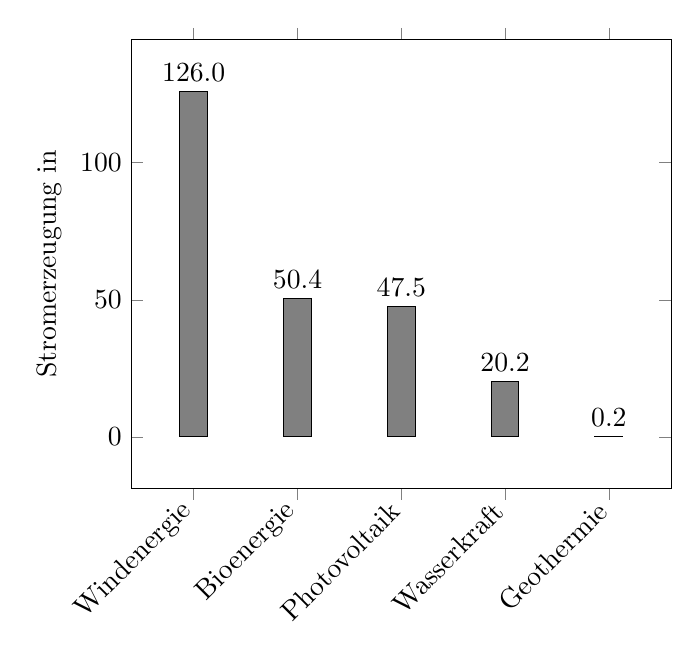
\begin{tikzpicture}
		\begin{axis}[
		ybar,
		enlargelimits=0.15,											% äüßerste bar plots nicht am Limit der x-Achse
		ylabel={Stromerzeugung in \si{\twh}},
		symbolic x coords={Windenergie,
			Bioenergie,
			Photovoltaik,
			Wasserkraft,
			Geothermie 
		},
		xtick=data,
		nodes near coords,											% Zahlen auf den bar plots
		nodes near coords align={vertical},
		nodes near coords style={/pgf/number format/.cd,fixed,fixed zerofill,precision=1},
		x tick label style={rotate=45,anchor=east},
		]
		\addplot[black,fill=black!50!white] coordinates {
			(Windenergie,126.0) (Bioenergie,50.4) (Photovoltaik,47.5) (Wasserkraft,20.2) (Geothermie,0.2)
		};
		\end{axis}
	\end{tikzpicture}
	\caption{Verteilung der Bruttostromerzeugung aus erneuerbaren Energien nach Erzeugungsart im Jahr 2019 \parencite{BWE2020}; \textit{Eigene Darstellung}}
	\label{fig:ee-gen_total}
\end{figure}

Biogasanlagen produzieren mit \SI{29.2}{\twh} den Großteil der Bruttostromerzeugung aus Bioenergie, während Biomethan mit einer Erzeugung von \SI{2.7}{\twh} eine untergeordnete Rolle spielt (s. Abb. \ref{fig:ee-gen_biomass}). \parencite{BWE2020} 

% Bar Chart - Biomasse Bruttostromerzeugung 2019

\begin{figure}[H]
	\centering
	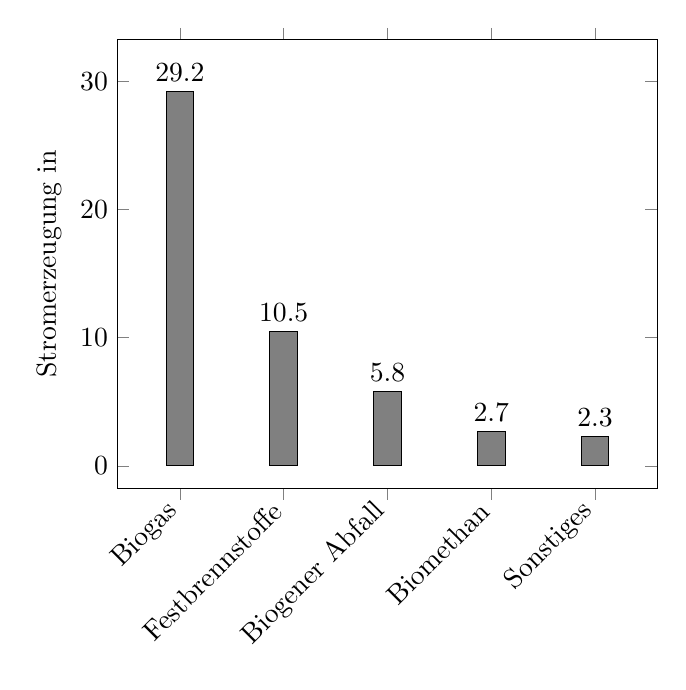
\begin{tikzpicture}
		\begin{axis}[
		ybar,
		enlargelimits=0.15,											% äüßerste bar plots nicht am Limit der x-Achse
		ylabel={Stromerzeugung in \SI{}{\twh}},
		symbolic x coords={Biogas,
			Festbrennstoffe,
			Biogener Abfall,
			Biomethan,
			Sonstiges 
		},
		xtick=data,
		nodes near coords,											% Zahlen auf den bar plots
		nodes near coords align={vertical},
		x tick label style={rotate=45,anchor=east},
		]
		\addplot[black,fill=black!50!white] coordinates {
			(Biogas,29.2) (Festbrennstoffe,10.5) (Biogener Abfall,5.8)
			(Biomethan,2.7) (Sonstiges,2.3)
		};
		\end{axis}
	\end{tikzpicture}
	\caption{Verteilung der Bruttostromerzeugung aus Bioenergie nach Brennstoffart im Jahr 2019 \parencite{BWE2020}; \textit{Eigene Darstellung}}
	\label{fig:ee-gen_biomass}
\end{figure}

Ende 2019 waren in Deutschland mehr als \SI{9000}{\relax} Biogas- und Biomethananlagen mit einer Kraftwerksleistung von \SI{5.9}{\gw} und \SI{0.6}{\gw} am Netz (s. Abb. \ref{fig:ee-cap_biogas}). Seit dem \gls{EEG} \SI{2012}{\relax} geht der Zubau von Biogasanlagen deutlich langsamer voran als in den vorangegangenen Jahren. Stattdessen erfolgt aufgrund der Einführung der Flexibilitätsprämie in erster Linie eine Erweiterung bestehender Biogasanlagen, um Flexibilität bereitstellen zu können. \parencite{BWE2020} \parencite{DanielGromke2019}

\begin{tikzpicture}
%%% Bar Plot
\begin{axis}[
	ybar stacked,
	ymin=-1500,ymax=7000,
	bar width=10pt,
	legend style={
		at={(0.5,-0.20)},
		anchor=east,
		legend columns=1,
		draw=none},
	legend cell align={left},
	ylabel={Leistung in \si{\giga\watt}},
	symbolic x coords={
		2005,
		2006,
		2007,
		2008,
		2009,
		2010,
		2011,
		2012,
		2013,
		2014,
		2015,
		2016,
		2017,
		2018,
		2019
},
	xtick=data,
	xticklabels={
		2005,,,,,
		2010,,,,,
		2015,,,,
		2019
	},
	%x tick label style={rotate=45,anchor=east},
	ytick={-1000, 0, 1000, 2000, 3000, 4000, 5000, 6000},
	yticklabels={, 0,, 2,, 4,, 6}
	]
\addplot+[ybar, draw=black, pattern=north east lines] plot coordinates {(2005,665) (2006,1000) (2007,1226) (2008,1419) (2009,2520) (2010,3015) (2011,3837) (2012,4212) (2013,4317) (2014,4380) (2015,4601) (2016,4780) (2017,5173) (2018,5597) (2019,5901) };
\addplot+[ybar, draw=black, fill=black!50!white] plot coordinates {(2005,0) (2006,0) (2007,6) (2008,16) (2009,18) (2010,96) (2011,218) (2012,256) (2013,383) (2014,603) (2015,614) (2016,653) (2017,567) (2018,557) (2019,558) };
\legend{\strut Inst. Leistung Biogas, \strut Inst. Leistung Biomethan}
\end{axis}

%%% Line Plot
\begin{axis}[
	ymin=-150,ymax=700,
	axis y line*=right,
	legend style={
		at={(0.5,-0.20)},
		anchor=west,
		legend columns=1,
		draw=none},
	legend cell align={left},
	ylabel={Zubau in \si{\mega\watt}},
	symbolic x coords={
		2005,
		2006,
		2007,
		2008,
		2009,
		2010,
		2011,
		2012,
		2013,
		2014,
		2015,
		2016,
		2017,
		2018,
		2019
},
	xtick=data,
	xticklabels={,,,,,,,,,,,,,,,,,,,,,,,,,,,,,},
	ytick={-100, 0, 100, 200, 300, 400, 500, 600},
	yticklabels={, 0,, 200,, 400,, 600}
	]
\addplot[sharp plot, draw=black, very thick] plot coordinates {(2005,0) (2006,0) (2007,6) (2008,10) (2009,2) (2010,78) (2011,122) (2012,38) (2013,127) (2014,220) (2015,11) (2016,39) (2017,-86) (2018,-10) (2019,1)};
\legend{\strut Nettozubau Biomethan}
\end{axis}
\end{tikzpicture}

In den Jahren 2010 bis \SI{2014}{\relax} ist der Ausbau von Biomethananlagen am größten. Ab dem \gls{EEG} \SI{2014}{\relax} (s. Kap. \ref{chap:law_theo}) kommt es zu einem starken Einbruch in dem Zubau von Kraftwerksleistung und in den Jahren \SI{2017}{\relax} und \SI{2018}{\relax} ist dieser mit einem Rückbau von \SI{86}{\mw} bzw. \SI{10}{\mw} sogar negativ (s. Abb. \ref{fig:ee-cap_biogas}). Hier zeigt sich, dass die Anreize seit Neuauflage des \gls{EEG} \SI{2014}{\relax} nicht ausreichen, um einen Ausbau der Biomethankapazitäten zu erreichen. \parencite{BWE2020} \smallskip

Insgesamt wird deutlich, dass ein Großteil der bestehenden Anlagenleistung an Biogasanlagen innerhalb des nächsten Jahrzehnts seine Förderung nach dem \gls{EEG} verlieren wird. Es ist somit dringend geboten alternative Erlösströme zu finden, die über dem Niveau einer reinen Direktvermarktung an der Strombörse liegen. Da das niedrige Preisniveau der Strommarkterlöse ansonsten zu einem Rückgang der Stromerzeugung aus Biogas- und Biomethananlagen führen würde. Deshalb soll diese Arbeit aufzeigen, ob die Biogasaufbereitung zu Biomethan eine solche Möglichkeit darstellen kann.

% ToDo: Wie viel kann man an der Strombörse verdienen?


\subsubsection{Wärme und Kälte}

Der Endenergieverbrauch in dem Sektor Wärme und Kälte entsprach im Jahr 2019 \SI{13.4}{\twh} an Biogas und \SI{3.3}{\twh} an Biomethan. Dies entspricht einem Anteil von \SI{1.1}{\percent} bzw. \SI{0.3}{\percent} an dem Gesamtendenergieverbrauch in der Erzeugung von Wärme und Kälte von \SI{1216.7}{\twh}. Ein Großteil der erneuerbaren Wärmeerzeugung von insgesamt \SI{152.0}{\twh} aus Bioenergie stammt hingegen aus Festbrennstoffen. \parencite{BWE2020}\smallskip

Unter den richtigen Rahmenbedingungen kann davon ausgegangen werden, dass der Einsatz von Biomethan in Zukunft zunehmen wird. Vor allem kann Biomethan eine stärke Rolle in der Erbringung von industrieller Prozesswärme bei hohen Temperaturen und bei der Spitzenlastdeckung übernehmen. Insgesamt wird ein Einsatz von \SI{18}{\twh} bis \SI{35}{\twh} an Biomethan an der Wärme- und Kälteproduktion im Jahr 2050 prognostiziert, wenn die rechtlichen Rahmen hierfür geschaffen werden. \parencite{dena2017}


\subsubsection{Verkehr}

Mit einem Endenergieverbrauch von \SI{0.7}{\twh} an Biomethan und einer gesamten Erzeugung aus erneuerbaren Energie von \SI{36.9}{\twh} im Verkehrssektor im Jahr 2019 ist der Anteil am Gesamtmarkt von \SI{656.8}{\twh} sehr gering. \parencite{BWE2020} \smallskip

Zukünftig kann Biomethan in Form von Bio-\gls{LNG} im Schwerlast-, Schiffs- und Flugverkehr eine bedeutendere Rolle übernehmen. Da in diesem Bereich voraussichtlich Verbrennungsmotoren für lange Zeit die dominierende Antriebstechnologie bleiben werden. \parencite{dena2017}